\documentclass{article}
\usepackage[utf8]{inputenc}
\usepackage[utf8]{inputenc}

\usepackage[top=2cm, bottom=3.5cm, left=2.5cm, right=2.5cm]{geometry}

\usepackage{enumitem}
\usepackage{booktabs}
\usepackage[T1]{fontenc}
\usepackage{float}

\usepackage{graphicx}
\usepackage{epstopdf}

%
% The following macro is used to generate the header.
% Arguments are
% Course, Semester+Year, Homework number, Due Date, Student
%
\newcommand{\homework}[5]{
   \thispagestyle{plain}
   \newpage
   \noindent
   \begin{center}
   \framebox{
      \vbox{\vspace{2mm}
    \hbox to 6.28in { {\bf #1 \hfill #2} }
       \vspace{6mm}
       \hbox to 6.28in { {\Large \hfill Homework \##3 - Due date: #4\hfill} }
       \vspace{4mm}
       \hbox to 6.28in { {\hfill Student: #5} }
      \vspace{2mm}}
   }
   \end{center}
}

% Style of Greek letters
\renewcommand{\phi}{\varphi}
\renewcommand{\epsilon}{\varepsilon}

\usepackage{titlesec}
\renewcommand{\thesection}{\Roman{section}}
\titleformat{\section}
  {\mdseries\scshape\Large}{\Large{\mdseries\scshape Part }\thesection\ -\ }{0pt}{}
\titleformat{\subsection}
  {\mdseries\scshape\large}{\large{\mdseries\scshape Problem }\thesubsection\ -\ }{0pt}{}
\newcommand{\problem}{\subsection}

%%%%%%%%%%%%%%%%%%%%%% Macros EPFL-MLO %%%%%%%%%%%%%%%%%%%%%%%
\usepackage{amssymb,amsmath,amsthm,dsfont}

% Indicator function
\usepackage{bbm}
\providecommand{\ind}[1]{\mathbbm{1}_{\{#1\}}}

\providecommand{\lin}[1]{\ensuremath{\left\langle #1 \right\rangle}}
\providecommand{\abs}[1]{\ensuremath{\left\lvert#1\right\rvert}}
\providecommand{\norm}[1]{\ensuremath{\left\lVert#1\right\rVert}}

\providecommand{\refLE}[1]{\ensuremath{\stackrel{(\ref{#1})}{\leq}}}
\providecommand{\refEQ}[1]{\ensuremath{\stackrel{(\ref{#1})}{=}}}
\providecommand{\refGE}[1]{\ensuremath{\stackrel{(\ref{#1})}{\geq}}}
\providecommand{\refID}[1]{\ensuremath{\stackrel{(\ref{#1})}{\equiv}}}

  % basic sets
  \providecommand{\R}{\mathbb{R}} % Reals
  \providecommand{\N}{\mathbb{N}} % Naturals
  
  % random variables
  \DeclareMathOperator{\E}{{\mathbb E}}
  %\providecommand{\E}[1]{{\mathbb E}\left.#1\right. }     %expectation
  \providecommand{\Eb}[1]{\ensuremath{\E \left[#1\right] }} %expectation, with brackets
  \providecommand{\EE}[2]{\E_{#1} \! #2 }      %expectation  
  \providecommand{\EEb}[2]{\ensuremath{\E_{#1}\!\! \left[#2\right] }} %expectation,  with brackets
  \providecommand{\prob}[1]{\ensuremath{{\rm Pr}\left[#1\right] } }
  \providecommand{\Prob}[2]{\ensuremath{{\rm Pr}_{#1}\left[#2\right] } }
  \providecommand{\P}[1]{\ensuremath{{\rm Pr}\left.#1\right. }}
  \providecommand{\Pb}[1]{\ensuremath{{\rm Pr}\left[#1\right] }}
  \providecommand{\PP}[2]{\ensuremath{{\rm Pr}_{#1}\left[#2\right] }}
  \providecommand{\PPb}[2]{\ensuremath{{\rm Pr}_{#1}\left[#2\right] }}
  
  \newcommand\independent{\protect\mathpalette{\protect\independenT}{\perp}}
  \def\independenT#1#2{\mathrel{\rlap{$#1#2$}\mkern2mu{#1#2}}}

  % operators
  \DeclareMathOperator*{\argmin}{arg\,min}
  \DeclareMathOperator*{\argmax}{arg\,max}
  \DeclareMathOperator*{\supp}{supp}
  \DeclareMathOperator*{\diag}{diag}
  \DeclareMathOperator*{\Tr}{Tr}
  
  % bold vectors
  \providecommand{\0}{\mathbf{0}}
  \providecommand{\1}{\mathbf{1}}
  \renewcommand{\aa}{\mathbf{a}}
  \providecommand{\bb}{\mathbf{b}}
  \providecommand{\cc}{\mathbf{c}}
  \providecommand{\dd}{\mathbf{d}}
  \providecommand{\ee}{\mathbf{e}}
  \providecommand{\ff}{\mathbf{f}}
  \let\ggg\gg
  \renewcommand{\gg}{\mathbf{g}}
  \providecommand{\gv}{\mathbf{g}}
  \providecommand{\hh}{\mathbf{h}}
  \providecommand{\ii}{\mathbf{i}}
  \providecommand{\jj}{\mathbf{j}}
  \providecommand{\kk}{\mathbf{k}}
  \let\lll\ll
  \renewcommand{\ll}{\mathbf{l}}
  \providecommand{\mm}{\mathbf{m}}
  \providecommand{\nn}{\mathbf{n}}
  \providecommand{\oo}{\mathbf{o}}
  \providecommand{\pp}{\mathbf{p}}
  \providecommand{\qq}{\mathbf{q}}
  \providecommand{\rr}{\mathbf{r}}
  \renewcommand{\ss}{\mathbf{s}}
  \providecommand{\tt}{\mathbf{t}}
  \providecommand{\uu}{\mathbf{u}}
  \providecommand{\vv}{\mathbf{v}}
  \providecommand{\ww}{\mathbf{w}}
  \providecommand{\xx}{\mathbf{x}}
  \providecommand{\yy}{\mathbf{y}}
  \providecommand{\zz}{\mathbf{z}}
  
  % bold matrices
  \providecommand{\mA}{\mathbf{A}}
  \providecommand{\mB}{\mathbf{B}}
  \providecommand{\mC}{\mathbf{C}}
  \providecommand{\mD}{\mathbf{D}}
  \providecommand{\mE}{\mathbf{E}}
  \providecommand{\mF}{\mathbf{F}}
  \providecommand{\mG}{\mathbf{G}}
  \providecommand{\mH}{\mathbf{H}}
  \providecommand{\mI}{\mathbf{I}}
  \providecommand{\mJ}{\mathbf{J}}
  \providecommand{\mK}{\mathbf{K}}
  \providecommand{\mL}{\mathbf{L}}
  \providecommand{\mM}{\mathbf{M}}
  \providecommand{\mN}{\mathbf{N}}
  \providecommand{\mO}{\mathbf{O}}
  \providecommand{\mP}{\mathbf{P}}
  \providecommand{\mQ}{\mathbf{Q}}
  \providecommand{\mR}{\mathbf{R}}
  \providecommand{\mS}{\mathbf{S}}
  \providecommand{\mT}{\mathbf{T}}
  \providecommand{\mU}{\mathbf{U}}
  \providecommand{\mV}{\mathbf{V}}
  \providecommand{\mW}{\mathbf{W}}
  \providecommand{\mX}{\mathbf{X}}
  \providecommand{\mY}{\mathbf{Y}}
  \providecommand{\mZ}{\mathbf{Z}}
  \providecommand{\mLambda}{\mathbf{\Lambda}}
  
  % caligraphic
  \providecommand{\cA}{\mathcal{A}}
  \providecommand{\cB}{\mathcal{B}}
  \providecommand{\cC}{\mathcal{C}}
  \providecommand{\cD}{\mathcal{D}}
  \providecommand{\cE}{\mathcal{E}}
  \providecommand{\cF}{\mathcal{F}}
  \providecommand{\cG}{\mathcal{G}}
  \providecommand{\cH}{\mathcal{H}}
  \providecommand{\cI}{\mathcal{I}}
  \providecommand{\cJ}{\mathcal{J}}
  \providecommand{\cK}{\mathcal{K}}
  \providecommand{\cL}{\mathcal{L}}
  \providecommand{\cM}{\mathcal{M}}
  \providecommand{\cN}{\mathcal{N}}
  \providecommand{\cO}{\mathcal{O}}
  \providecommand{\cP}{\mathcal{P}}
  \providecommand{\cQ}{\mathcal{Q}}
  \providecommand{\cR}{\mathcal{R}}
  \providecommand{\cS}{\mathcal{S}}
  \providecommand{\cT}{\mathcal{T}}
  \providecommand{\cU}{\mathcal{U}}
  \providecommand{\cV}{\mathcal{V}}
  \providecommand{\cX}{\mathcal{X}}
  \providecommand{\cY}{\mathcal{Y}}
  \providecommand{\cW}{\mathcal{W}}
  \providecommand{\cZ}{\mathcal{Z}}

% Commenting
\RequirePackage[colorinlistoftodos,bordercolor=orange,backgroundcolor=orange!20,linecolor=orange,textsize=scriptsize]{todonotes}
\providecommand{\comment}[2]{\todo[inline,caption={}]{\textbf{#1: }#2}}%
\providecommand{\inlinecomment}[3]{%
  %\@getnewcolor%
  %\edef\@tempa{\@colstring}%
  {\color{#1}#2: #3}}%
\newcommand\commenter[2]%
{%
  \expandafter\newcommand\csname i#1\endcsname[1]{\inlinecomment{#2}{#1}{##1}}
  \expandafter\newcommand\csname #1\endcsname[1]{\comment{#1}{##1}}
}

% Use these for theorems, lemmas, proofs, etc.
\newtheorem{proposition}{Proposition}
\newtheorem{lemma}{Lemma}
\newtheorem{corollary}[lemma]{Corollary}
%\newtheorem{conjecture}[lemma]{Conjecture}
\newtheorem{definition}{Definition}
\newtheorem{remark}[lemma]{Remark}
\newtheorem{assumption}{Assumption}
\newtheorem{theorem}[lemma]{Theorem}
\newtheorem{example}[lemma]{Example}

\newtheorem{claim}{Claim}
\newtheorem{fact}{Fact}

\newcommand{\propositionautorefname}{Proposition}
\newcommand{\lemmaautorefname}{Lemma}
\newcommand{\corollaryautorefname}{Corollary}
\newcommand{\definitionautorefname}{Definition}
\newcommand{\remarkautorefname}{Remark}
\newcommand{\assumptionautorefname}{Assumption}
\newcommand{\theoremautorefname}{Theorem}
\newcommand{\exampleautorefname}{Example}
\newcommand{\claimautorefname}{Claim}
\newcommand{\factautorefname}{Fact}

\definecolor{mydarkblue}{rgb}{0,0.08,0.45}
\usepackage[colorlinks=true,linkcolor=blue]{hyperref} 
\hypersetup{ %
    colorlinks=true,
    linkcolor=mydarkblue,
    citecolor=mydarkblue,
    filecolor=mydarkblue,
    urlcolor=mydarkblue
}
\usepackage[capitalize,noabbrev]{cleveref}


\usepackage{url}
\def\UrlBreaks{\do\/\do-}

\usepackage[round]{natbib}
\renewcommand{\cite}[1]{\citep{#1}}



\begin{document}

\homework{Mathematics of Data}{Fall 2019}{3}{6\textsuperscript{th} December 2019}{Oriol Barbany Mayor}

\problem{Multiclass Classification}
\subsection*{Part I - Theory}
\begin{enumerate}[label=1.I.\arabic*]
    \item Assuming that the samples are statistically independent, we can write the likelihood of observing vector $\bb \in \{1, \dots, C\}^n$ as
    \begin{align}
        \Pr (\bb | A , X) = \prod_{i=1}^{n} \prod_{j=1}^{C} \Pr (b_i = j | \aa_i, X)^{\ind{b_i = j}} = \prod_{i=1}^{n} \prod_{j=1}^{C} \left( \frac{e^{\aa_i^T \xx_j}}{\sum_{k=1}^{C} e^{\aa_i^T \xx_j}} \right)^{\ind{b_i = j}}
    \end{align}
    
    The log-likelihood thus have the form
    \begin{align}
        \ell(X) := \log \Pr (\bb | A , X) = \sum_{i=1}^{n} \sum_{j=1}^{C} \ind{b_i = j} \left( \aa_i^T \xx_j - \log \sum_{k=1}^{C} e^{\aa_i^T \xx_j} \right) = \sum_{i=1}^{n} \left( \aa_i^T \xx_{b_i} - \log \sum_{k=1}^{C} e^{\aa_i^T \xx_{k}} \right)
    \end{align}
    and the maximum likelihood estimator of $X$ is given by
    \begin{align}
        \hat{X}_{ML} \in \argmax_X \{ \ell(X) \} = \argmin_X \left\lbrace -\ell(X) = \sum_{i=1}^{n} \left( \log \sum_{k=1}^{C} e^{\aa_i^T \xx_{k}} - \aa_i^T \xx_{b_i} \right) := f(X) \right\rbrace
    \end{align}
    
    \item
    \begin{align}
        \nabla_X f(X) = [\nabla_{\xx_1} f(X), \cdots, \nabla_{\xx_C} f(X)]
    \end{align}
    
    Let's find the value of this gradient at one of the columns, namely $j$
    \begin{align}
        \nabla_{\xx_j} f(X) = \sum_{i=1}^{n} \left( \frac{\aa_i e^{\aa_i^T \xx_{j}} }{ \sum_{k=1}^{C} e^{\aa_i^T \xx_{k}}} - \aa_i \ind{b_i = j}\right)
    \end{align}
    
    In matrix notation, we can write
    \begin{align}
        \nabla_X f(X) = A^T (Z \exp{(A X)} - Y)
    \end{align}
    where $Z \in \R^{n \times n}$ has entries
    \begin{align*}
        Z_{i,j} = \begin{cases}
        \frac{1}{\sum_{k=1}^{C} e^{\aa_i^T \xx_{k}}} &\text{if }i=j \\
        0 &\text{otherwise}
        \end{cases},
    \end{align*}
    $Y\in \{0,1\}^{n\times C}$ is a matrix whose rows are the one-hot encoding of $b_i$ and $\text{exp}$ is applied entry-wise.
    \item Proving that $f$ is convex is equivalent to showing that its Hessian is PSD.
    \begin{align}
        \nabla^2 f(X) = \sum_{i=1}^{n} \Sigma_i \otimes \aa_i \aa_i^T
    \end{align}
    
    \begin{fact}
        If $D, E \succeq 0$, then $D \otimes E \succeq 0$.
        \label{fact1}
    \end{fact}
    
    So to proof that $ \nabla^2 f(X)$ is PSD, it's only left to show that $D,E \succeq 0 \Longrightarrow D+E \succeq 0$ and $\aa_i \aa_i^T, \Sigma_i \succeq 0$. By definition,
    \begin{align}
        D \succeq 0 \Longleftrightarrow \zz^T D \zz \geq 0 \quad \forall \zz
    \end{align}
    so if $D,E \succeq 0$,
    \begin{align}
        \zz^T (D + E) \zz = \zz^T D \zz + \zz^T E \zz \geq \zz^T E \zz \geq 0\quad \forall \zz \Longleftrightarrow D+E \succeq 0
        \label{eq:sum_psd}
    \end{align}

    Note that $\aa_i \aa_i^T$ is indeed PSD, since
    \begin{align}
        \zz^T \aa_i \aa_i^T \zz = \norm{\aa_i^T \zz}^2 \geq 0 \quad \forall \zz \Longleftrightarrow \aa_i \aa_i^T \succeq 0
    \end{align}
    where the inequality follows by non-negativity of the norm.
    
    Finally, to show that $\Sigma_i$ is also PSD, note that $\Sigma_i = \Lambda - \mathbf{s}_i \mathbf{s}_i^T $ with $\mathbf{s}_i =[\sigma_{i1},\dots, \sigma_{iC}]^T$ and $\Lambda=\text{diag}(\mathbf{s}_i)$. By definition of positive semidefiniteness,
    \begin{align}
        \zz^T \Sigma_i \zz &= \zz^T (\Lambda - \mathbf{s}_i \mathbf{s}_i^T)\zz = \zz^T \Lambda \zz - |\lin{\mathbf{s}_i, \zz}|^2 \\
        &:= \sum_{j=1}^{C} z_j^2 \sigma_{ij} - \left(\sum_{j=1}^{C} z_j \sigma_{ij}\right)^2 \\
        &\geq \sum_{j=1}^{C} z_j^2 \sigma_{ij} - \sum_{j=1}^{C} \left( z_j \sigma_{ij}\right)^2 &&\text{by convexity of $(\cdot)^2$}\\
        &= \sum_{j=1}^{C} z_j^2 (\sigma_{ij} - \sigma_{ij}^2) \geq \sum_{j=1}^{C} z_j^2 &&\text{since $0\leq \sigma_{ij} \leq 1$}\\
        &:= \norm{\zz} \geq 0 &&\text{by non-negativity of norm}
    \end{align}
    
    The proof concludes by applying Fact \ref{fact1} to show that $\Sigma_i \otimes \aa_i \aa_i^T \succeq 0 \quad \forall i$ and by again applying \eqref{eq:sum_psd} $n$ times to show $\sum_i \Sigma_i + \aa_i \aa_i^T \succeq 0$.
    \item We can upperbound the largest eigenvalue of the matrix $\aa_i \aa_i^T$ as
    \begin{align}
        \lambda_{\max} (\aa_i \aa_i^T) &= \max_{\xx \in \R^n} \frac{\xx^T \aa_i \aa_i^T \xx}{\xx^T \xx} = \max_{\xx \in \R^n}\frac{\xx^T \aa_i \aa_i^T \xx}{\xx^T \xx} = \max_{\xx \in \R^n}\frac{\lin{\xx, \aa_i}^2}{\norm{\xx}^2} \\
        &\leq \max_{\xx \in \R^n} \frac{\norm{\xx}^2 \norm{\aa_i}^2}{\norm{\xx}^2}  = \norm{\aa_i}^2
    \end{align}
    where inequality follows from Cauchy-Schwarz.
    
    For the matrix $\Sigma_i$, we can use the inequality
    \begin{align}
        \lambda_{\max} (\Sigma_i) \leq \max_j \sum_{k=1}^C |\Sigma_{i_{jk}}| = \max_j \sum_{k=1}^C |\Sigma_{i_{jk}}| = \max_j \sigma_{ij} \left[(1-\sigma_{ij})+\sum_{k=1, k\neq j}^C \sigma_{ik} \right]
    \end{align}
    where I use $1 \geq \sigma_{ij} \geq 0 \quad \forall i,j \in \{1,\dots, C\}$. Note that $1-\sigma_{ij}=\sum_{k=1, k\neq j}^C \sigma_{ik}$ so
    \begin{align}
        \lambda_{\max} (\Sigma_i) \leq \max_j 2 \sigma_{ij} (1-\sigma_{ij}) \leq \frac{1}{2}
    \end{align}
    where the last inequality follows by maximizing the resulting expression, i.e.
    \begin{align}
        \frac{\partial}{\partial \sigma_{ij}} 2 \sigma_{ij} (1-\sigma_{ij}) = 2(1- 2 \sigma_{ij}) = 0 \Longleftrightarrow \sigma_{ij} = \frac{1}{2}
    \end{align}
    
    \begin{fact}
        If $D, E \succeq 0$, then $\lambda_{\max}(D \otimes E) = \lambda_{\max}(D)\lambda_{\max}(E)$.
        \label{fact2}
    \end{fact}
    
    Using Fact \ref{fact2}, we have that
    \begin{align}
         \lambda_{\max} (\Sigma_i \otimes \aa_i \aa_i^T) = \lambda_{\max} (\Sigma_i ) \lambda_{\max}(\aa_i \aa_i^T) \leq \frac{1}{2}\lambda_{\max}(\aa_i \aa_i^T) \leq \frac{\norm{\aa_i}^2}{2}
    \end{align}
    
    \begin{lemma}
        For two matrices $A, B \in \R^{n\times n}$, $\lambda_{\max}(A+B)\leq \lambda_{\max}(A)+\lambda_{\max}(B)$
        \label{lemma:1}
    \end{lemma}
    \begin{proof}
        We can express the maximum eigenvalue of the matrix $A+B$ as
        \begin{align}
            \lambda_{\max}(A+B)=\max_{\xx \in \R^n }\frac{\xx ^T (A+B)\xx}{\norm{\xx}^2} \leq \max_{\xx \in \R^n }\frac{\xx ^T A\xx}{\norm{\xx}^2}+\max_{\xx \in \R^n }\frac{\xx ^T B\xx}{\norm{\xx}^2}=\lambda_{\max}(A)+\lambda_{\max}(B)
        \end{align}
    \end{proof}
    
    Finally, applying Lemma \ref{lemma:1} $n-1$ times,
    \begin{align}
        \lambda_{\max}(\nabla^2 f) \leq \sum_{i=1}^n \frac{\norm{\aa_i}^2}{2} := \frac{\norm{A}^2_F}{2}=L
    \end{align}
    
    \item For $g(\xx):=\norm{\xx}_1$,
    \begin{align}
        \text{prox}_{\lambda g}(\zz) := \argmin_{\yy \in \R^d} \left\lbrace \lambda \norm{\yy}_1 + \frac{1}{2} \norm{\yy - \zz}^2_2\right\rbrace = \argmin_{\yy \in \R^d} \left\lbrace \sum_{i=1}^d \lambda |y_i| + \frac{1}{2} (y_i-z_i)^2\right\rbrace
    \end{align}
    
    So using the first order optimality condition,
    \begin{align}
       \frac{\partial}{\partial y_j} \left\lbrace \sum_{i=1}^d \lambda |y_i| + \frac{1}{2} (y_i-z_i)^2 \right\rbrace =  \lambda s + (y_j-z_j) = 0
    \end{align}
    where $s \in \partial |y_j |$. We can distinguish, the following cases, where $s$ is taken to be 0 in the case $y_j=0$:
    \begin{align}
        y_j =
        \begin{cases}
            z_j - \lambda &\text{if $y_j>0$, so $z_j > \lambda$} \\
            z_j + \lambda &\text{if $y_j<0$, so $z_j < -\lambda$} \\
            0 &\text{if }y_j=0
        \end{cases}
    \end{align}
    which can be summarised as $y_j = \max{(|z_j|-\lambda, 0)}\text{sign}(z_j)$. Finally, we have
    \begin{align}
         \nabla_{\yy} \left\lbrace \sum_{i=1}^d \lambda |y_i| + \frac{1}{2} (y_i-z_i)^2 \right\rbrace = 0 \Longleftrightarrow \yy = \max{(|\zz|-\lambda, \0)}\circ \text{sign}(\zz)
    \end{align}
    where the operators $\max, \text{sign}$ and $|\cdot|$ are applied coordinate-wise. So the resulting proximal operator is
    \begin{align}
        \text{prox}_{\lambda g}(\zz) = \max{(|\zz|-\lambda, \0)}\circ 
        \text{sign}(\zz)
    \end{align}
    
    \item For $g(\xx):=\frac{1}{2}\norm{\xx}_2^2$,
    \begin{align}
        \text{prox}_{\lambda g}(\zz) := \argmin_{\yy \in \R^d} \left\lbrace \lambda \frac{1}{2}\norm{\yy}_2^2 + \frac{1}{2} \norm{\yy - \zz}^2_2\right\rbrace
    \end{align}
    
    Again equating the gradient to zero,
    \begin{align}
        \nabla_{\yy} \left\lbrace \lambda \frac{1}{2}\norm{\yy}_2^2 + \frac{1}{2} \norm{\yy - \zz}^2_2\right\rbrace = \lambda \yy + (\yy - \zz) = 0 \Longleftrightarrow \yy = \frac{\zz}{1+\lambda}
    \end{align}
    so the proximal operator in this case is
    \begin{align}
        \text{prox}_{\lambda g}(\zz) = \frac{\zz}{1+\lambda}
    \end{align}
\end{enumerate}

\subsection*{Part II - Handwritten Digit Classification}

\subsubsection*{Discussion of the convergence plots}
As we can see in Figures \ref{fig:conv_l1} and \ref{fig:conv_l2}, the convergence with ISTA algorithm is very slow for both $\ell_1$ and $\ell_2$ regularized logistic regression. Note that for the latter case it offers the poorest performance.

Regarding the Stochastic Proximal method, we observe a flat behavior for the $\ell_1$ regularization and a better performance that the deterministic ISTA algorithm for $\ell_2$ regularization. Differently from the deterministic algorithms, the x axis of the stochastic plot is the number of epochs, so it would correspond to one iteration of a deterministic method. Hence, \texttt{PROX-SG} has effectively half as many iterations as the deterministic methods.

Note that the previous algorithms offer a very slow convergence since the step size is chosen to be the Lipschitz constant of the gradients for each of the problems. This is of the order of $10^5$, hence the resulting step size is $10^{-5}$ which explains the flat behavior of the convergence curves.

For this reason, accelerated algorithms are specially suited in this case. As expected, FISTA performs better than any other algorithm for these problems and its restarted version is equivalent until the occurrence of the first ripple. By construction, the restarted version is monotonically decreasing and converges faster in the number of iterations.

\begin{figure}[ht]
    \centering
    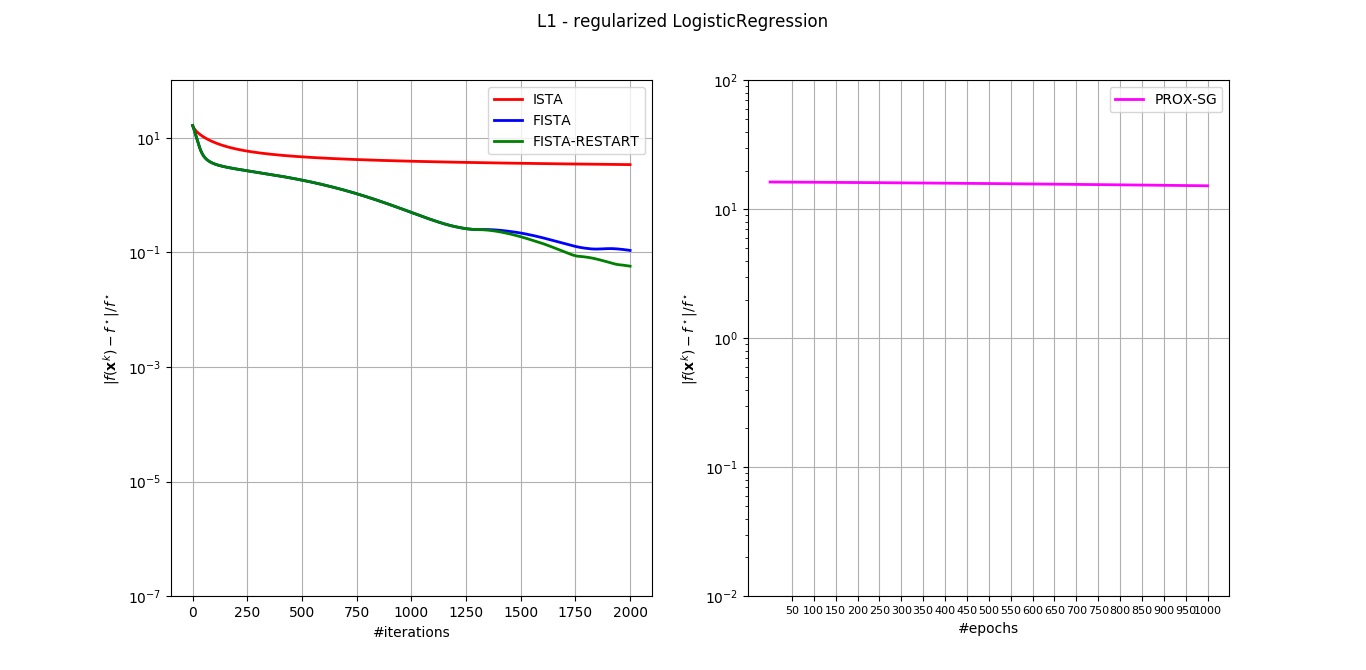
\includegraphics[trim={2.5cm 0.5cm 3cm 0},clip, width=.9\textwidth]{img/convergence_l1.png}
    \caption{Convergence of $\ell_1$-regularized Logistic regression}
    \label{fig:conv_l1}
\end{figure}
\begin{figure}[ht]
    \centering
    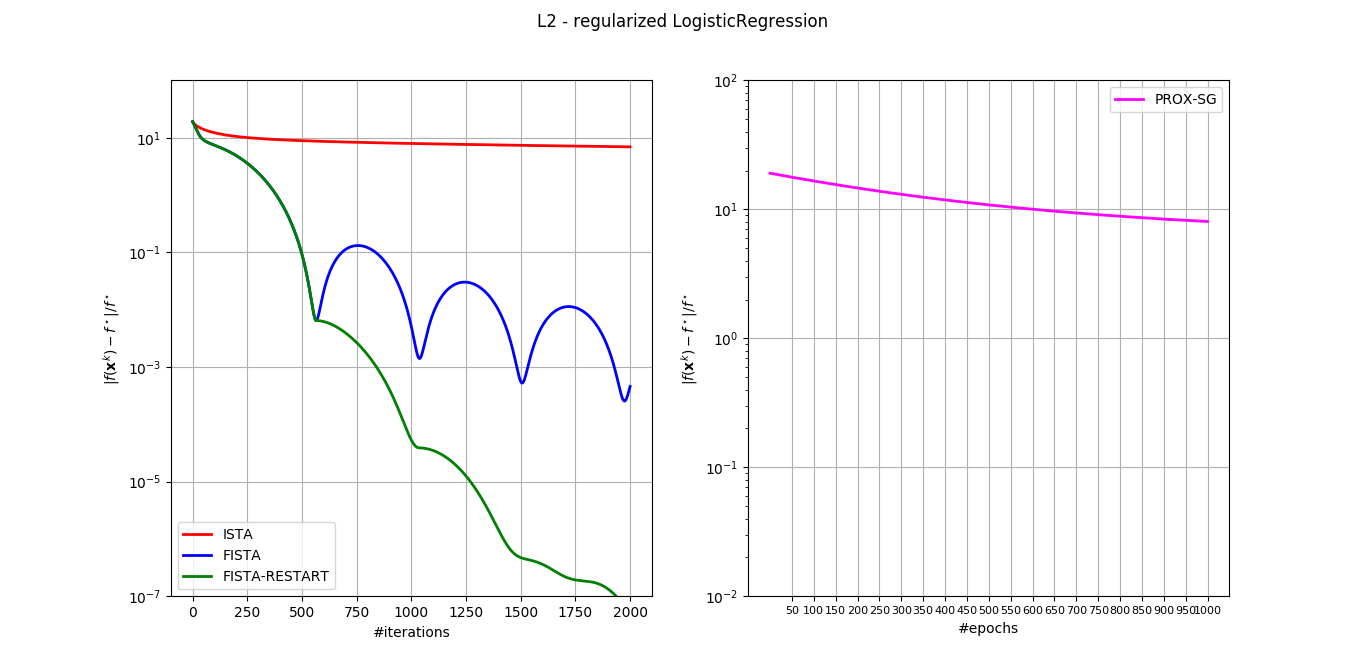
\includegraphics[trim={2.5cm 0.5cm 3cm 0},clip, width=.9\textwidth]{img/convergence_l2.png}
    \caption{Convergence of $\ell_2$-regularized Logistic regression}
    \label{fig:conv_l2}
\end{figure}

\subsubsection*{Theoretical convergence rates}
As mentioned in the previous section, the slow convergence is due to the large Lipschitz constant $L$ of the gradient of the objective function, which translates into a very little step size. The theoretical convergence rates of both ISTA and FISTA algorithms have the form
\begin{align}
    \frac{F(\xx^k) - F^*}{F^*} \leq 
    \begin{cases}
        \frac{F^* L R_0^2}{2(k+2)} &\text{for ISTA algorithm} \\
        \frac{2 F^* L R_0^2}{(k+2)^2} &\text{for FISTA algorithm}
    \end{cases}
    \label{eq:theo}
\end{align}
where $R_0 = \norm{\xx_0 - \xx^*}$. These bounds are depicted as dashed lines in Figure \ref{fig:theo}. Here we can see that, even if the convergence is in general very slow as discussed in the previous section, the empirical results are below the theoretical bounds, which have a large value due to the huge $L$ factor in \eqref{eq:theo}.

\begin{figure}[ht]
    \centering
    \begin{minipage}{.45\textwidth}
        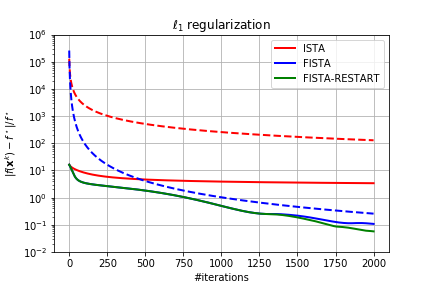
\includegraphics[width=\textwidth]{img/l1_reg.png}
    \end{minipage}
    \begin{minipage}{.45\textwidth}
        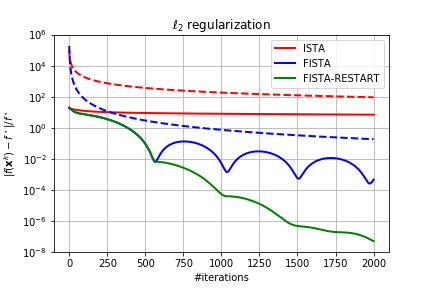
\includegraphics[width=\textwidth]{img/l2_reg.png}
    \end{minipage}
    \caption{Comparison against theoretical convergence rates}
    \label{fig:theo}
\end{figure}

\subsubsection*{Digit features}
Figure \ref{fig:vis} depicts the feature matrices obtained by running FISTA with gradient restart. Specially for the case of $\ell_2$ regularization, we can see similarities between each class and the depicted values. This can be easily seen for classes 0 and 1.

\begin{figure}[ht]
    \centering
    \begin{minipage}{.9\textwidth}
        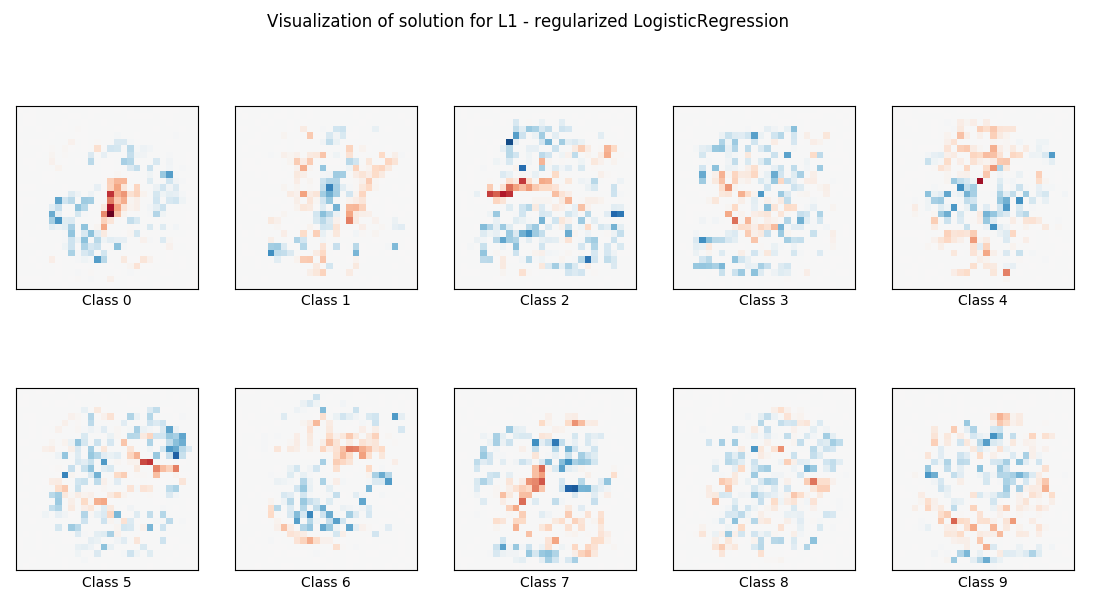
\includegraphics[trim={3.5cm 2cm 3cm 0},clip, width=\textwidth]{img/visual_l1.png}
    \end{minipage}
    \begin{minipage}{.9\textwidth}
        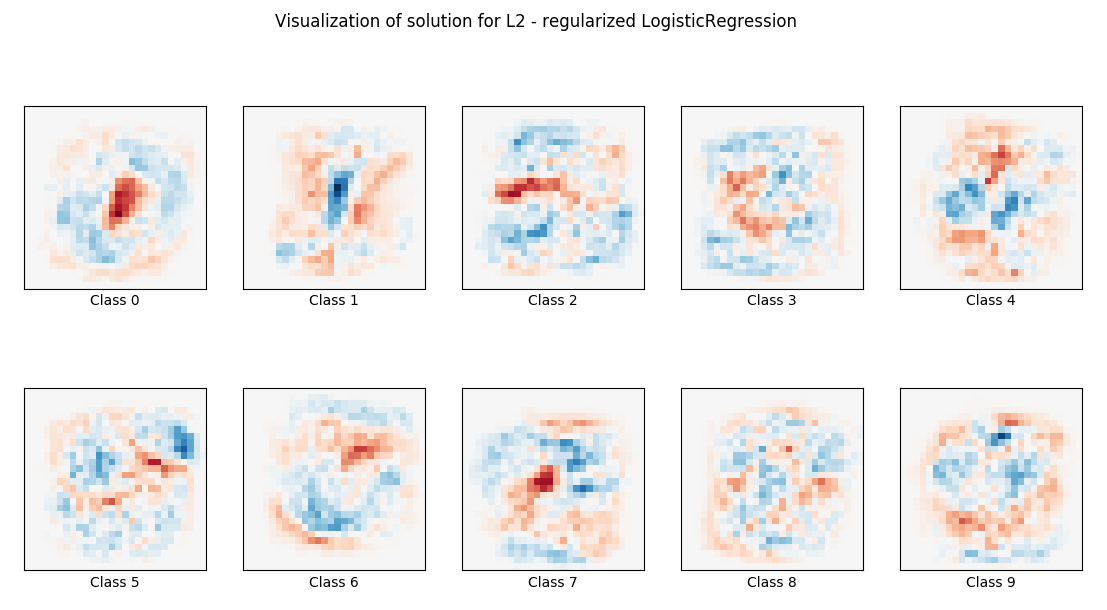
\includegraphics[trim={3.5cm 2cm 3cm 0},clip,width=\textwidth]{img/visual_l2.png}
    \end{minipage}
    \caption{Visualization of the feature matrices}
    \label{fig:vis}
\end{figure}

\subsubsection*{Comparison against Neural Network}
The test accuracies of both regularization versions of the Logistic Regression formulation are presented in Table \ref{tab:acc} along the test accuracy of a Neural Network. The tested model for Logistic regression is the one obtained by FISTA with gradient scheme restart for both $\ell_1$ and $\ell_2$ regularization, while the Neural Network is a 3-layer perceptron with ReLU activation functions.

As seen in Table \ref{tab:acc}, one can intuit that the Logistic Regression model has not as many expressive power as the Neural Network. The universal approximation theorem states that a 1-hidden-layer Neural Network with enough hidden units and a non-polynomial activation function can approximate a continuous function arbitrarily well. The theorem may not hold by the \textit{enough hidden units} condition, the same reasoning applies. Nevertheless, in this case we don't have a wide Neural Network but a one deeper that only one layer which increments the expressive power.

On the other hand, one can understand the Logistic Regression formulation as a one-layer neural network, i.e. no hidden layers, and with softmax activation function. Note that this activation function is continuous and can be arbitrarily well approximated using a Taylor series and there is no hidden layer. So in any case the general approximation theorem holds in this case.

\begin{table}[ht]
    \centering
    \begin{tabular}{ccc}
        \toprule
        $\ell_1-$regularized Logistic Regression &  $\ell_2-$regularized Logistic Regression & Neural Network\\
        \midrule
        89.20\% & 89.89\% & 94.70\% \\
        \bottomrule
    \end{tabular}
    \caption{Test accuracies for each setup}
    \label{tab:acc}
\end{table}

\problem{Image Reconstruction}
\begin{enumerate}[label=2.\arabic*]
    \item 
    \begin{enumerate}[label=\alph*)]
        \item 
        \begin{align}
            \nabla_{\boldsymbol{\alpha}}f(\boldsymbol{\alpha}) :=\nabla_{\boldsymbol{\alpha}} \left\lbrace \frac{1}{2}\norm{\bb - P_{\Omega} W^T \boldsymbol{\alpha}}_2^2 \right\rbrace = W P_{\Omega}^T (P_{\Omega} W^T \boldsymbol{\alpha} - \bb)
        \end{align}
        
        \begin{align}
            \nabla_{\xx}f(\xx) := \nabla_{\xx} \left\lbrace \frac{1}{2}\norm{\bb - P_{\Omega} \xx}_2^2 + \lambda_{\text{TV}}\norm{\xx}_{\text{TV}} \right\rbrace = P_{\Omega}^T (P_{\Omega} \xx - \bb) 
        \end{align}
        \item 
        \begin{align}
            \norm{\nabla_{\boldsymbol{\alpha}}f(\boldsymbol{\alpha}) - \nabla_{\boldsymbol{\alpha}}f(\boldsymbol{\beta})} &= \norm{W P_{\Omega}^T P_{\Omega} W^T(\boldsymbol{\alpha} - \boldsymbol{\beta})} \leq \norm{W P_{\Omega}^T P_{\Omega} W^T} \norm{\boldsymbol{\alpha} - \boldsymbol{\beta}} \\
            &:= L_{\ell_1} \norm{\boldsymbol{\alpha} - \boldsymbol{\beta}} \leq L \norm{\xx - \yy}
        \end{align}
        where the first inequality follows by definition of the spectral norm. 
        
        \begin{align}
            \norm{\nabla_{\xx} f(\xx) - \nabla_{\xx} f(\yy)} = \norm{P_{\Omega} ^TP_{\Omega} (\xx - \yy)} \leq \norm{P_{\Omega} ^TP_{\Omega}}\norm{\xx - \yy} := L_{TV}\norm{\xx - \yy} \leq L \norm{\xx - \yy}
        \end{align}
    
    A valid upper bound in both cases is $L=1$, which follows by noting that $P_{\Omega}$ is a projection that selects some coordinates without altering its values and the Wavelet transform defines an orthonormal basis. Summing up, both the matrices $P_{\Omega}^T P_{\Omega}$ and $W P_{\Omega}^T P_{\Omega} W^T$ will be diagonal with entries 1 in those coordinates selected by $P_{\Omega}$ and 0 otherwise. Hence, it's trivial to see that the maximum eigenvalue (and thus the spectral norm of these matrices) will be 1.
    \end{enumerate}
    \item 
    A parameter sweep over $\lambda_1$ and $\lambda_{\text{TV}}$ is depicted in Figure \ref{fig:lambda} against the Peak signal-to-noise ratio (PSNR) of the reconstructed image taking the original one as a reference. Each reconstruction has been obtained by running 200 iterations of FISTA. The higher the PSNR the better, and this can be seen in Figure \ref{fig:psnr_tv}.
    
    \begin{figure}[ht]
        \centering
        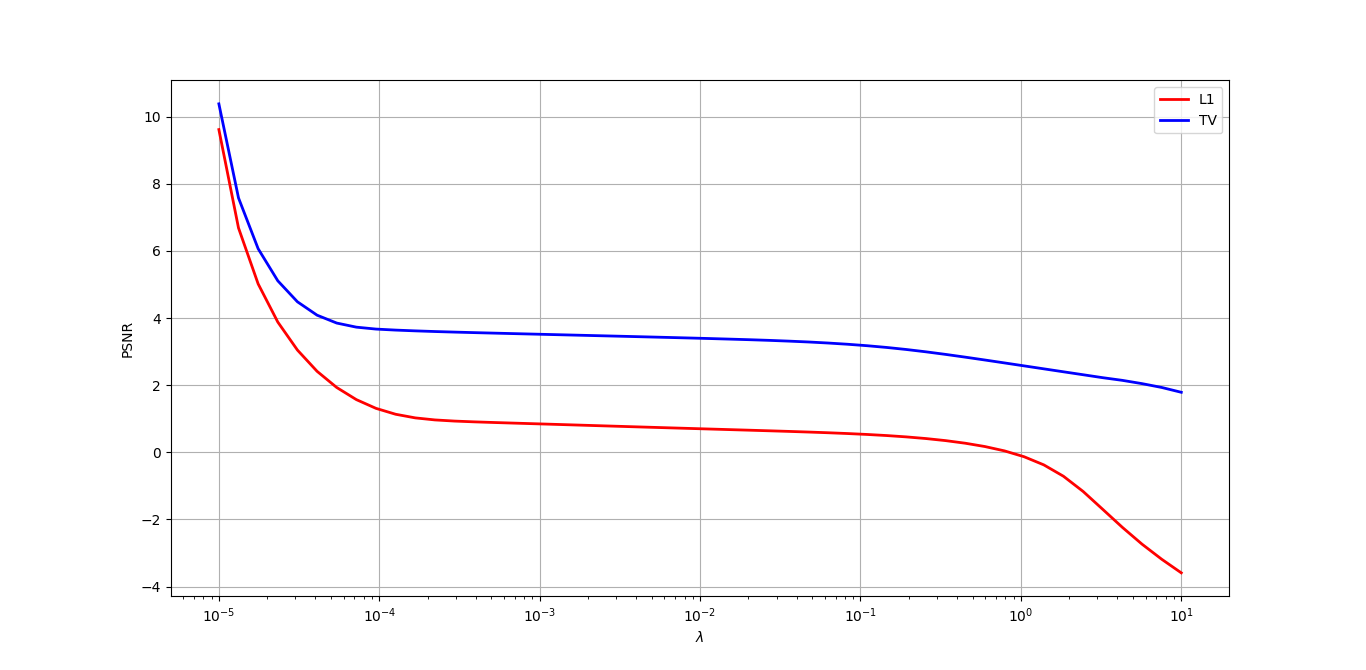
\includegraphics[trim={3cm 0.5cm 3cm 2cm},clip, width=.6\textwidth]{img/lambda_sweep.png}
        \caption{PSNR as a function of $\lambda$, the penalty parameter}
        \label{fig:lambda}
    \end{figure}
    
    \begin{figure}[ht]
        \centering
        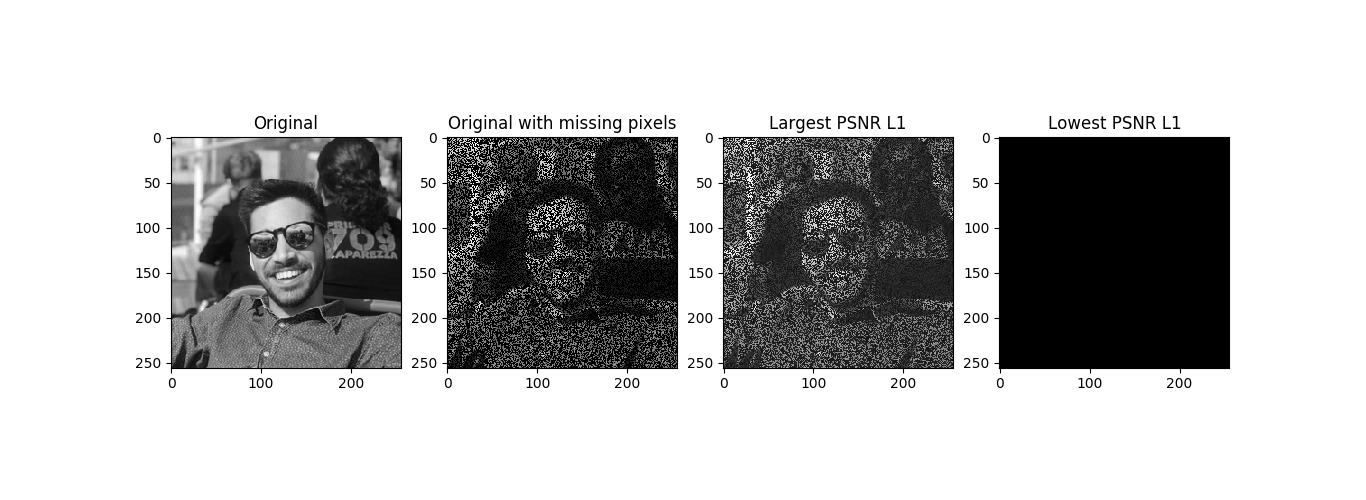
\includegraphics[trim={3.5cm 2cm 3cm 2.8cm},clip,width=\textwidth]{img/psnr_l1.png}
        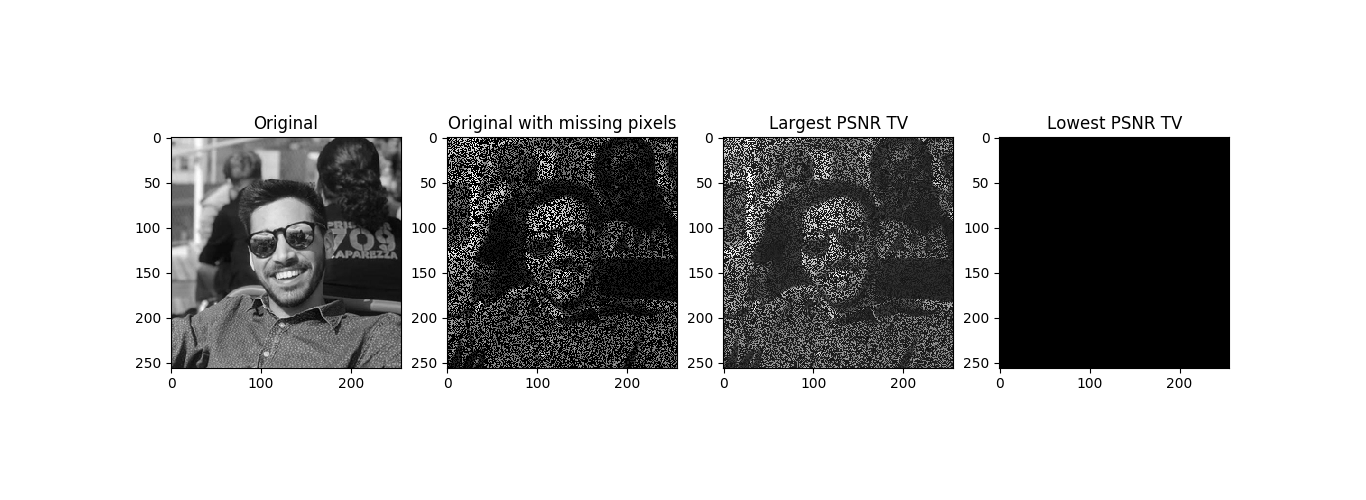
\includegraphics[trim={3.5cm 2cm 3cm 2.8cm},clip,width=\textwidth]{img/psnr_tv.png}
        \caption{Reconstructed images for $\ell_1$ and TV regularization with best and worst penalty}
        \label{fig:psnr_tv}
    \end{figure}
    \item
    \item
    
    We can see the reconstruction obtained for both $\ell_1$ and TV regularization after 500 steps in Figure \ref{fig:rec_500}, where apart from the original image and the original with missing pixels, we can see an error map of the reconstruction. In Figure \ref{fig:rec_nn}, the same results but for the unrolled proximal operator can be seen. Note that comparing the regularized methods, TV regularization obtains a better result in terms of the PSNR, the SSIM and also the time. Nevertheless, when compared with the neural network, even if the SSIM is the same, this latter has a slightly larger PSNR and the time to obtain the reconstruction is much lower. Nevertheless, the time accounts for the inference and not for the computation of the unrolled proximal model.
    
    \begin{figure}[ht]
        \centering
        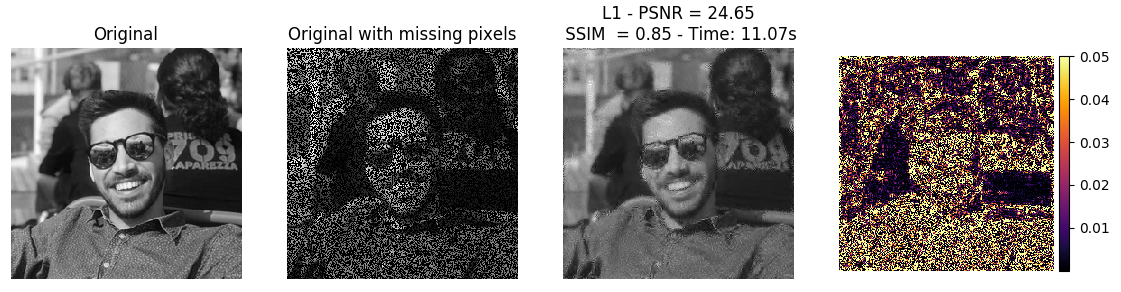
\includegraphics[trim={3.5cm 2cm 3cm 2cm},clip,width=\textwidth]{img/reconstruction_l1.png}
        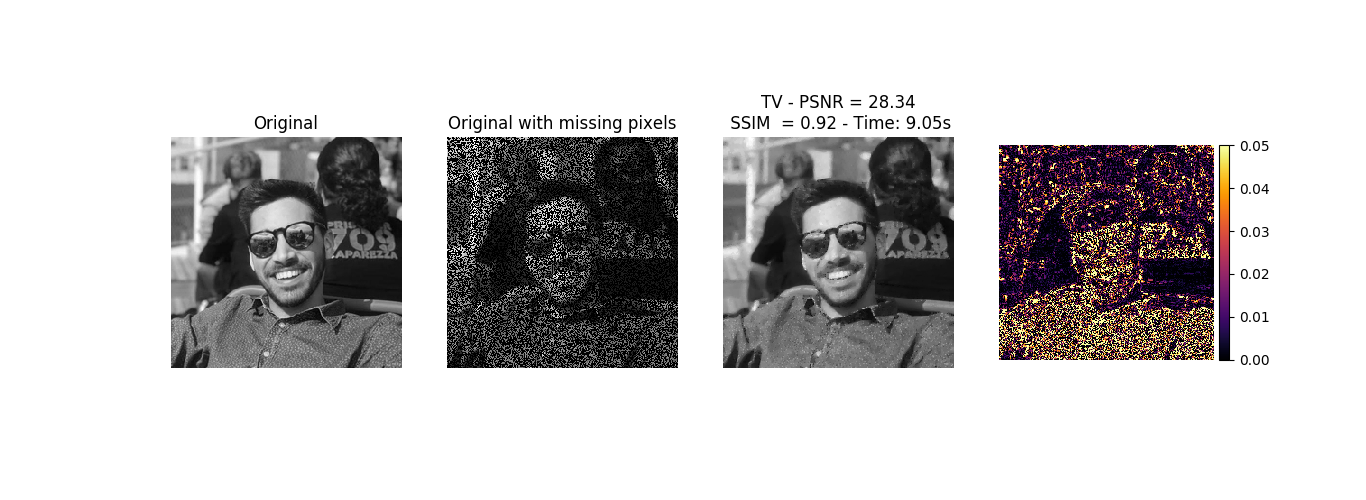
\includegraphics[trim={3.5cm 2cm 3cm 2cm},clip,width=\textwidth]{img/reconstruction_tv.png}
        \caption{Reconstruction with $\ell_1$ and TV-regularization and 500 iterations}
        \label{fig:rec_500}
    \end{figure}[ht]
    \begin{figure}
        \centering
        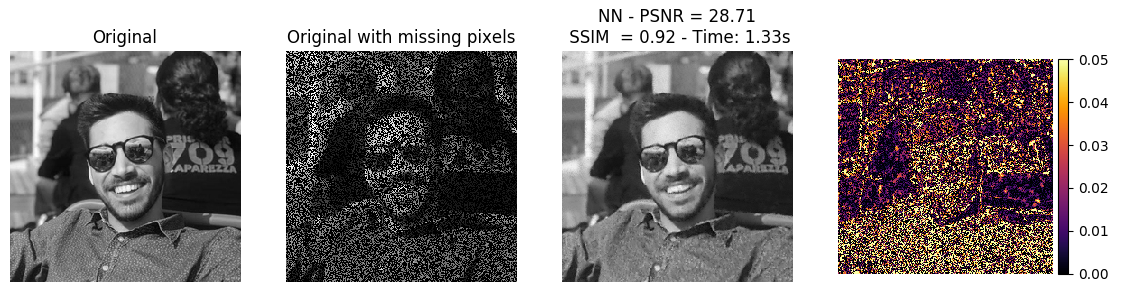
\includegraphics[trim={3.5cm 2cm 3cm 2cm},clip,width=\textwidth]{img/reconstruction_nn.png}
        \caption{Reconstruction using the trained unrolled proximal operator}
        \label{fig:rec_nn}
    \end{figure}
    
    For a fair comparison, Figure \ref{fig:5} show the results with only 5 iterations for the three methods considered before. Note that each iteration of the Neural Network costs roughly 200 times more that with the least squares problem formulation with either $\ell_1$ or TV regularization. These achieve very similar performance for only 5 iterations and are comparable with the trained unrolled proximal operator with 500 iterations, which still take less than half the time for five iterations of the Neural Network. Therefore, one would probably prefer TV regularization as the in-painting method.
    
    \begin{figure}[ht]
        \centering
        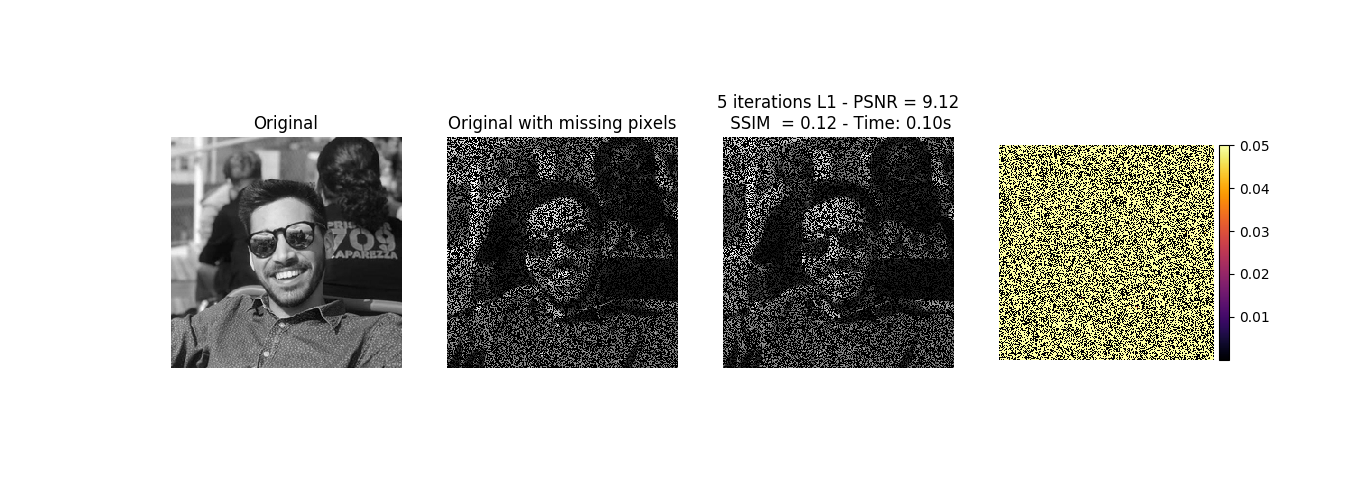
\includegraphics[trim={3.5cm 2cm 3cm 2cm},clip,width=\textwidth]{img/l1_5.png}
        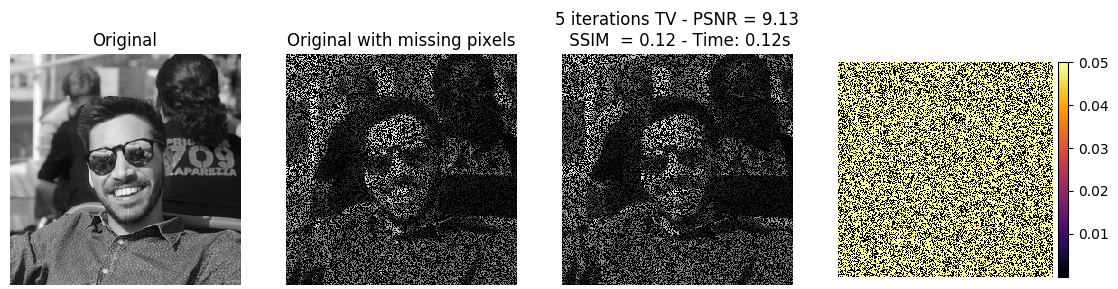
\includegraphics[trim={3.5cm 2cm 3cm 2cm},clip,width=\textwidth]{img/tv_5.png}
        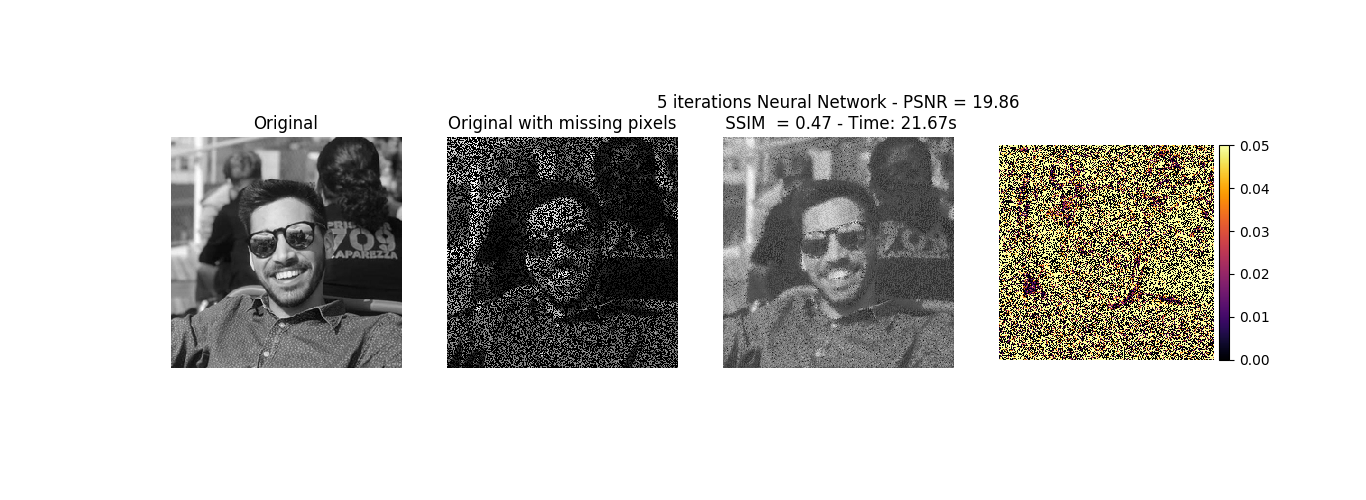
\includegraphics[trim={3.5cm 2cm 3cm 2cm},clip,width=\textwidth]{img/nn_5.png}
        \caption{Reconstructions using 5 iterations}
        \label{fig:5}
    \end{figure}
\end{enumerate}

\end{document}